\section{ESMF Superstructure:  Coupling and Control}
\label{sec:superclasses}

\subsection{Introduction}

In this section, we 
explain the classes involved in ESMF coupled applications, their 
relationships, and typical action sequences for coupled applications.  

\subsection{Design Goals and Considerations}

One of the primary goals of the ESMF project is to increase interoperability
across a range of Earth system modeling components.  As described in 
Section~\ref{sec:scope}, initially these 
components will be large scale, such as land models, ocean models, 
data assimilation systems and diagnostics packages.  As the 
framework evolves, we plan to utilize coupling services for smaller-scale 
tasks within model components, such as the transformation of data between the 
physics and dynamics in a spectral atmospheric model, or the creation 
of nested higher resolution regions within a coarser grid.  The ability to 
couple components at varying scales both flexibly and efficiently requires
careful design and implementation.  

The important aspects of this design are as follows:
\begin{itemize}
\item The coupling specification {\it is entirely external to gridded 
components involved in the coupling}, which makes it easier for the 
same gridded component to be reconfigured for a variety of scenarios.
\item Gridded components can be configured as for SPMD or MPMD and 
sequential or concurrent execution without changes to the gridded 
component code.  Changes to coupler or application code may be required. 
\item The ability to send data when it's ready from within a gridded
component allows computation to overlap with communication.  
\item It is not necessary to create return points from 
within the time iteration loop of a gridded component.  
\item Data may be sent between components without needing to 
be sent to a set of coupler DEs as an intermediate step.
\item The systematized approach to component scheduling will
enable a layer of tools for application configuration to be added to
the architecture in the future.
\end{itemize}

\subsection{Classes and Scoping}

There are restrictions on how objects within an application may be scoped
on a parallel platform.  There is only one application component defined 
for any application; it initially allocates resources and tracks 
application-wide information. 
The application component must be instantiated on 
any decomposition elements or DEs (see Section~\ref{sec:progmodel}) on 
which other components
within the application are defined.  This is true whether the 
application consists of a single executable or multiple 
executables.  

An ESMF coupled application typically involves an application component 
containing two or more gridded components that require an 
inter-component data exchange, and one or more coupling 
components.  However, any parent component that contains the appropriate 
subcomponents can manage their execution and coupling.  ESMF thereby
supports applications consisting of a hierarchy of coupled systems.

A coupler component must be instantiated on any DEs on which components
it will couple are defined.  This is consistent with an architectural
model in which communication is handled internal to components, and all
inter-component interactions are local (see Section~\ref{sec:strategies}).  
It is possible for
some portions of the functionality of a component to be restricted to
a subset of the DEs over which the component is defined.  For example, 
it may be computationally efficient for the computation of interpolation
weights to occur on a set of DEs not being used by any gridded components
in the application.  The coupler might define a subcomponent on those DEs 
specifically to handle that function.

A gridded component may exist across all DEs in the application.  When 
a set of gridded  components and a coupler all execute in sequence on 
the same set of DEs and are contained within an application running 
as a single executable we have a sequential execution SPMD configuration.  

Within an application, a gridded component may also reside on 
a subset of DEs.  These DEs may wholly coincide with, be wholly 
contained within or wholly contain another component.  Multiple gridded 
components may be defined as separate executables.  A typical 
concurrent execution MPMD configuration is one in which gridded components 
are defined on separate DEs running simultaneously as multiple 
executables.  

It is possible for ESMF applications to contain some component sets
that are executing sequentially and others that are executing concurrently.
We might have, for example, atmosphere and land components instantiated 
on the same set of 
DEs and running as one executable, ocean and sea ice 
components instantiated on a separate set of DEs and running as 
another executable, and a coupler and application component 
instantiated across all DEs.

Figure \ref{fig:couplerscaling} illustrates scoping of components
in a coupled, hierarchically structured application.  At the top level, 
a climate application consists of atmosphere and ocean components 
instantiated on mutually exclusive DE sets.  These components communicate 
via an atmosphere/ocean coupler defined on the union of their DEs.  
Scheduling is controlled by an application
component which is also defined across all DEs.  The atmosphere component
is similarly structured as a coupled application.  It consists of a 
physics component and a dynamics component, which are both distributed
across all the atmospheric DEs.  A physics/dynamics coupler controls
the data transpose between these subcomponents.  In this case, the
atmospheric component rather than the highest level application component
controls the coupling sequence.  

\begin{figure}
\caption[{Scoping of Components in a Coupled Application}]{A coupled
application may itself be composed of other coupled systems.}
\label{fig:couplerscaling}
\scalebox{0.7}{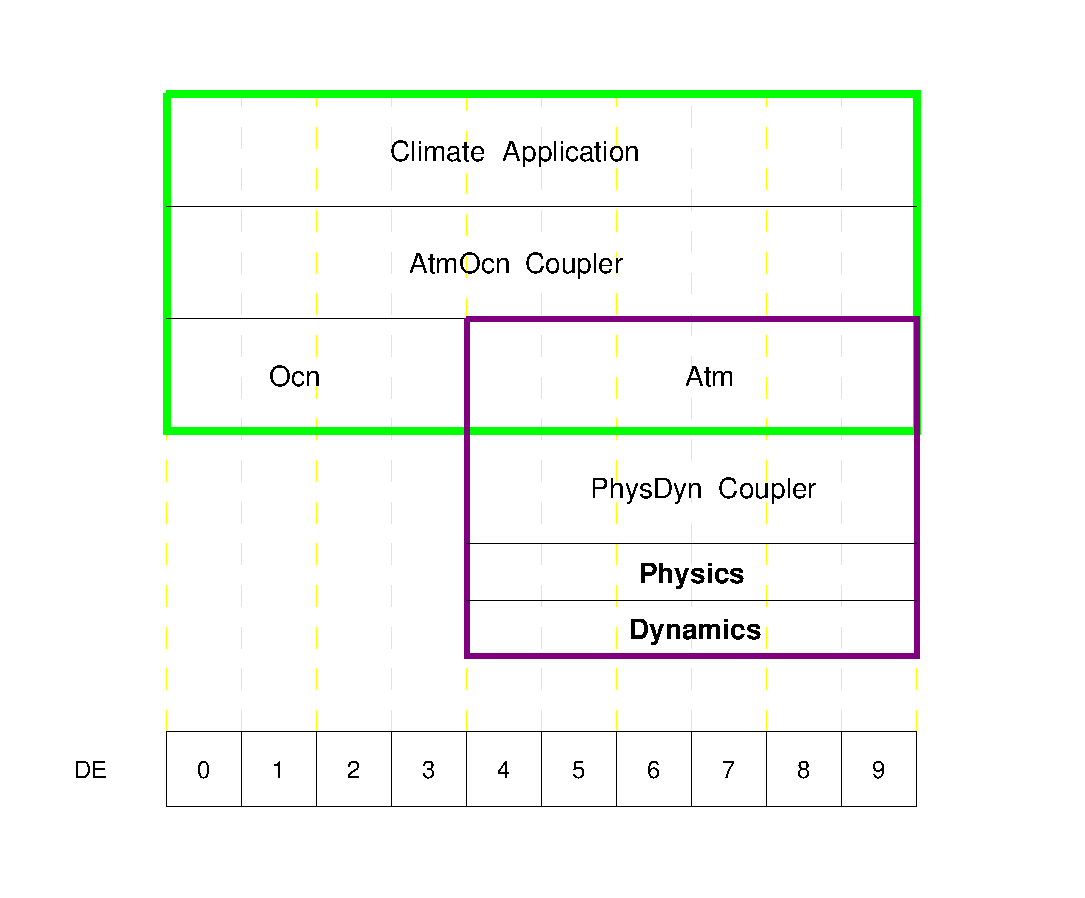
\includegraphics{CouplerScaling.eps}}
\end{figure}

\subsection{Flow of Control}

Gridded components have few responsibilities with respect to coupling
to other components.  They do not need to keep track of the data needed
by other components or to provide methods for inter-component 
grid transformations or transfers of data.  They {\it are} responsible for 
providing a description of all of the fields and data they
can export to other components, and for similarly providing a description 
of the data they require in order to run.  These descriptions are
embodied in the {\tt ESMF\_State} class, and the kind of data that they 
represent is identified by the {\tt type} attribute of that class, which can
have an {\tt ESMF\_IMPORT} or {\tt ESMF\_EXPORT} value.  The state class
includes metadata information as well as actual pointers to data 
locations.  The ESMF will provide methods that enable a user to add or
remove fields and data from States.  Gridded components are required to 
have an {\tt ESMF\_StateValidate} method that checks that initial or 
imported data is valid and complete.  

The coupler component produces a specification of the sequence of 
transforms that are necessary to effect communication between components, 
both scientific and computational, generic and user-defined.  The coupler 
returns these to the application in the form of a 
transform specification object, which contains a set of transforms 
along with associated sequencing restrictions.  Each transform has a
function pointer to a transform operation and may be bundled with 
associated data.

The application or parent component initiates the coupling and manages 
its scheduling.  It is responsible for instantiating the gridded components
that are exchanging data and the coupler, for setting up the desired 
sequencing, and making the calls to the methods of the components and 
coupler that effect the coupled exchange.  The parent may partition the 
transforms
for execution among the gridded components and the coupler, so that, for 
example, a data send or coupling transformation can occur while a gridded 
component is executing, without a need for the component to return to the
application level.  
To disable or rearrange the coupling sequence, a different set of function
pointers can be passed in to the component.
The gridded component call that executes the transform
is a generic {\tt ESMF\_StateTransform} call, which takes as arguments a
transform object and the component's import or export state. The
call {\tt ESMF\_StateValidate} ensures that all required transforms
have been performed by the data supplier and data is now available
for use.  For sequencing purposes, a {\tt ESMF\_StateTransformComplete} call
will return when the state data has been transformed and data
buffers are available to be reused.

\subsection{Flow of Data}

The design choices we have made enable the user to configure an ESMF
coupler so that data is transferred from one component to another, 
without requiring that it first be sent via message passing to the
coupler (or even necessarily
copied).  This is likely to be the most efficient way of performing 
inter-component coupling when the components are instantiated on different
DE sets.  However, if desired, an application can also be configured so that
data from a source component is sent to a distinct set of coupler 
DEs for processing before being sent to its destination.

\subsection{Implications for ESMF Users}

The above coupling architecture requires the following:
\begin{itemize}
\item Since gridded components will run on the same 
DEs as the application component, often in conjunction with a coupler, 
it is necessary to subroutinize
them and provide standard methods such as {\tt ESMF\_CompInit}, 
{\tt ESMF\_CompRun}, and {\tt ESMF\_CompFinalize}.  The {\tt ESMF\_CompRun}
command takes a time interval or number of timesteps as one of its 
arguments.
\item Gridded components must create ESMF import and export state 
structures.
\item The coupler component must define and return any transforms or 
sends that gridded components involved in a coupling interaction may 
perform.
\end{itemize}

\subsection{Examples}

Figure~\ref{fig:1waycoupling} shows the sequence of actions involved
in coupling an atmosphere to an ocean.  The vertical axis is time, positive
downward, and the horizontal axis shows the objects that are involved in the
exchange.  In this example, the coupling is one-way, so that the ocean 
receives data from the atmosphere but does not send any data back.  Atmosphere
and ocean components are configured for concurrent execution.

\begin{figure}
\label{fig:1waycoupling}
\caption[{Coupling Sequence}]{One-way coupling between an atmosphere and
ocean executing concurrently.}
\scalebox{0.70}{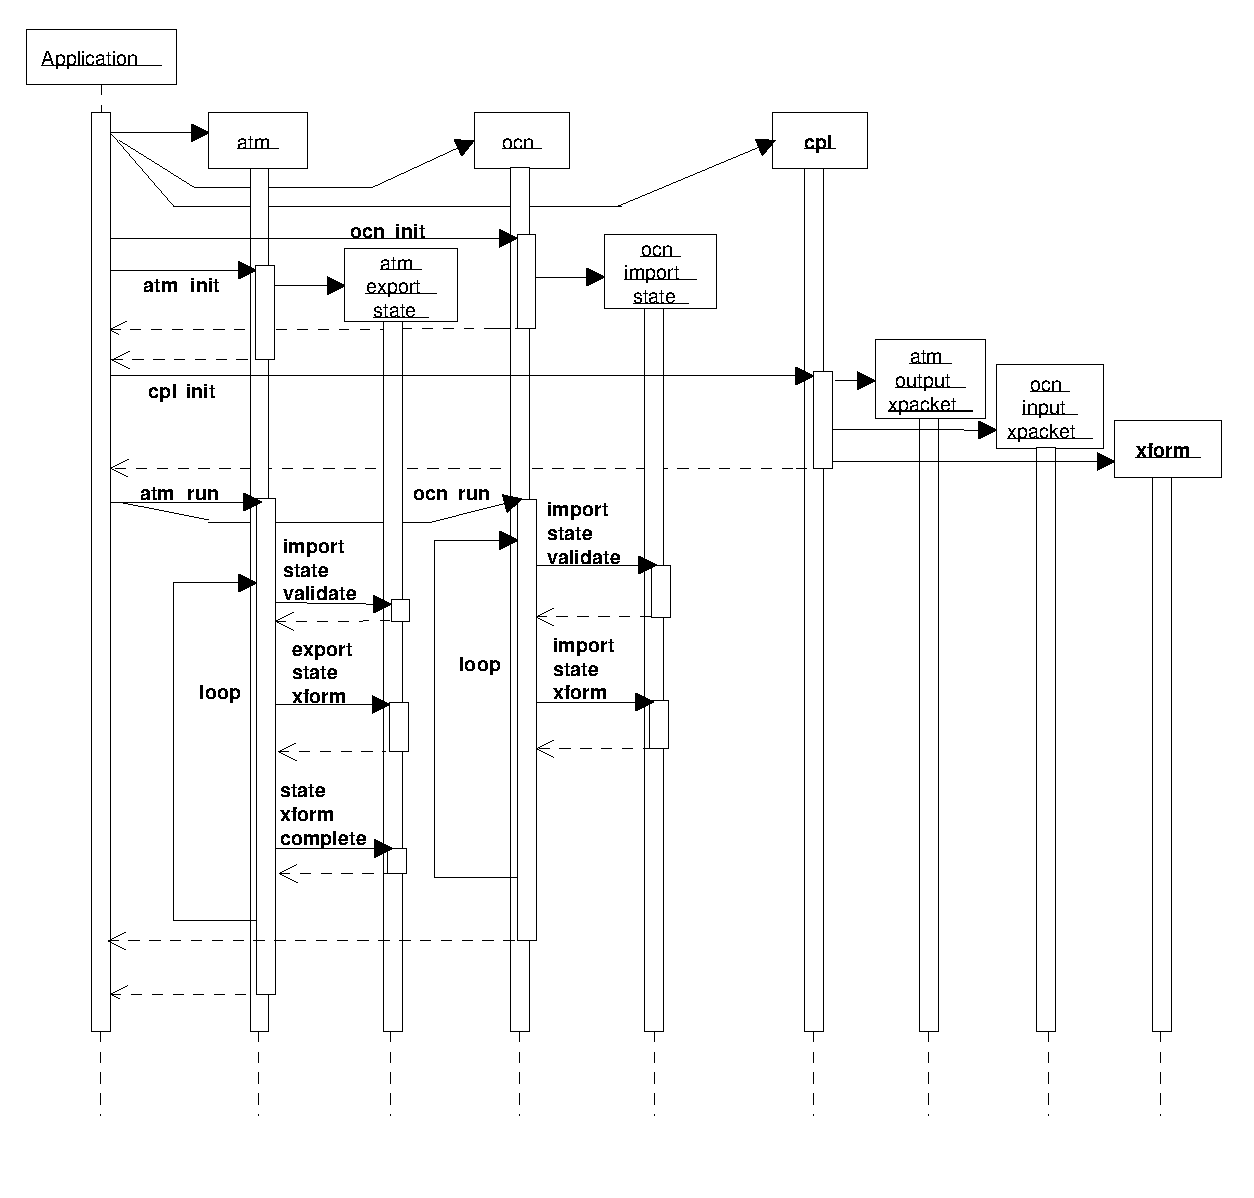
\includegraphics{OneWayCoupling.eps}}
\end{figure}

\subsection{Class Descriptions}

The following are brief descriptions of the objects involved in the
ESMF superstructure:

\subsubsection{Component (ESMF\_Comp)} 
\begin{description}
\item [Description] A Component is a functionally related computational entity that represents 
a large system.  
% \item [Function] The component base class defines a set of operations and
attributes common to all components.  These include methods such as:
initialize, run, finalize, get layout, get PE list, get status, and 
retrieve information, such as layout and status, about subcomponents.  
All couplers, gridded components and applications possess these methods. 
\end{description}

\subsubsection{Application Component (ESMF\_App)}
\begin{description} 
\item [Description] The ESMF\_App class is responsible for managing those 
functions that relate to an entire scientific application running under ESMF.
\item [Function]  The ESMF\_App initialize method 
must be called at the start of any user application operating under the framework, and
the ESMF\_App finalize method at its end.  At initialization the Application allocates and 
configures any resources needed to run the framework.  The ESMF\_App 
class can be queried 
for information such as an experiment name, model name, and run 
type (ESMF\_INIT, ESMF\_BRANCH, etc.).  
\end{description}

\subsubsection{Coupler Component (ESMF\_Coupler)}
\begin{description}
\item [Description] A Coupler is a user-customized type of Component that 
encompasses all the 
functionality needed to communicate data between two or more Components. 
\item [Function] A coupler has a coupling initiation method that defines and 
returns a sequence of transforms.
\end{description}

\subsubsection{Gridded Component (ESMF\_GComp)}
\label{sec:griddedcomponent} 
\begin{description}
\item [Description] A gridded component is a user-customized Component 
that typically represents a physical system discretized on some spatial grid.
\item [Function] The gridded component class has methods for writing 
fields and data to an import state and export state, for verifying that
these states are fully or partially complete, and for returning these
states.
\end{description}

\subsubsection{State (ESMF\_State)}
\begin{description}
\item [Description] A state is a description of a set of data that a 
gridded component either needs to run or can make available.  States
have a type attribute that can have values or {\tt ESMF\_IMPORT} or
{\tt ESMF\_EXPORT}.
\item [Function] A state has a state transform method that
takes as arguments a state and a function pointer to a transform.

\end{description}

\subsubsection{Transform (ESMF\_XForm)} 
\begin{description}
\item [Description] A transform acts on a state or other type of 
ESMF data.  It may relocate data, redistribute data, regrid data, 
change units, or any combination of these.  
\item [Function] Transforms have names and may have dependencies
or sequencing attributes. 

\end{description}







